We explore applications of {\sc Ludus} to problems commonly faced by game designers.

\subsection{Group versus round-robin tournament}

% Maybe explain the group tournament in more detail
The first experiment we ran was to determine the efficacy of our sampling method. To do this, we compared the win rates of identical decks in a complete round robin tournament (every combination of decks played) with the win rate in a tournament conducted by randomly grouping decks into groups of various sizes, and then playing every combination of the decks within those groups.

\begin{figure}[t]
	\centering
	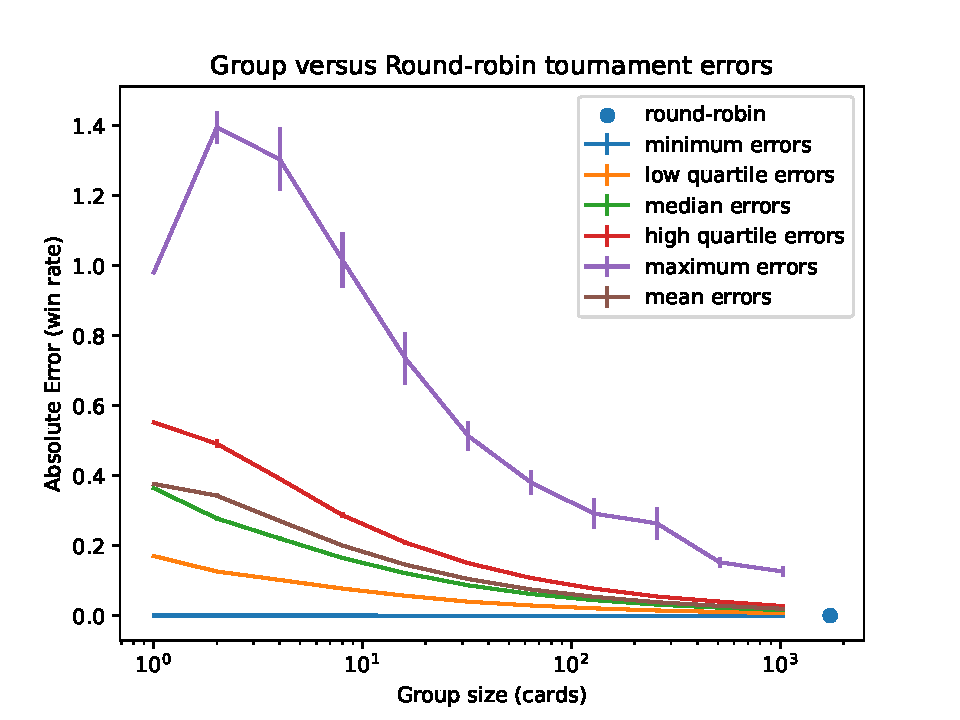
\includegraphics[width=0.9\columnwidth]{group_vs_rr_fig}
	\caption{Absolute value of the difference in win rate between a \textit{group tournament} of varying size and a full round-robin tournament of 1728 possible decks. %, along with error bars.
	}
	\label{fig:group_vs_rr}
\end{figure}

%% Table

We then compare the win rates of each deck in the group tournament versus the round robin tournament, and we can see that at a group size of 256, the mean error becomes negligible (about 0.0382). This is the group size we have chosen to use in the other experiments.

% Another table

 \subsection{Optimizing cards without special mechanics}

The next experiment optimized a set of four basic cards, with no extra mechanics. We hypothesized that the `optimal' solution in terms of the standard deviation metric would have 4 identical cards, because then there would be only one card and thus zero standard deviation in the win rate of one card. We also recognized, however, that due to the limited number of generations run by our genetic algorithm, there was no guarantee it would find this solution. This case seemed even more interesting from a game design perspective, as a game with only a single card is obviously an uninteresting game, so we would like to see what `almost-optimal' solutions appear for this setup. This observation also illustrates a case where the standard deviation metric fails to fully capture the qualities we wish to optimize in our game.

The results of this experiment illustrate a different failure case of our standard deviation metric, one that had not been predicted. The genetic algorithm quickly found the solution (5/3), (5/4), (8/3), (8/1), where ($a$,$b$) indicates a card with $a$ attack and $b$ health points. This solution had zero standard deviation. Why? Any pairing of these cards will result in both cards being killed. Thus, every game ends after one round in a tie, and so there is no variance in win rates amongst the decks. 

 \subsection{Optimizing only special mechanics}

The third experiment was to optimize twelve cards, each with a special mechanic. Each of these cards was assigned an intuitive value for its attack and health, as a game designer might do. We then optimized the stats that controlled the special mechanics of these cards. We were interested to see how feasible it is to optimize the game with these constraints, and how impactful the special mechanics would be for the overall balance of the game. The cards used in this experiment are described in Table~\ref{tab:special_cards}. The optimizer improved the win rate standard deviation from 0.0751 to 0.0589. 

\begin{table*}[t]
\centering
\begin{tabular}{||c c c c||} 
 \hline
 Card & Attack & Health & Variable special parameter (see Section~\ref{sec:ab-game-def})\\ [0.5ex] 
 \hline\hline
 Explode On Death & 2 & 1 & Damage dealt to enemies on death \\ 
 \hline
 Friendly Vampire & 1 & 3 & Amount of heath granted to ally \\
 \hline
 Grow On Damage & 0 & 5 & Attack gained per hit taken \\
 \hline
 Heal On Death & 1 & 2 & Health granted to allies on death \\
 \hline
 Health Donor & 1 & 4 & Percent of healing received that is split amongst allies \\
 \hline
 Ignore First Damage & 2 & 1 & Number of attacks which result in no damage taken \\
 \hline
 Morph Attack & 0 & 3 & N/A \\
 \hline
 Pain Splitter & 2 & 2 & Percent of damage taken that is split amongst allies \\
 \hline
 Rampage & 0 & 4 & Middle Age  \\
 \hline
 Survivalist & 2 & 2 & N/A \\
 \hline
 Threshold & 2 & 2 & Number of battles it must survive to damage all opponents on death \\
 \hline
 Time Bomb & 1 & 8 & Number of interactions before it will explode during the next battle \\ 
 \hline
\end{tabular}
\caption{Variable and set parameters for the \textit{optimize special parameters} experiment}
\label{tab:special_cards}
\end{table*}

\subsection{Optimizing all parameters} \label{sec:first_set}

After fixing the attack and health, and focusing solely on the special mechanics, the next logical experiment is to tune both the attack and health, as well as the special mechanics. To reduce the huge dimensionality of this experiment we selected only five cards to optimize. They are listed in Table~\ref{tab:first_set}.

% First Set
\begin{table*}[t]
\centering
\begin{tabular}{||c c c c||} 
 \hline
 Card & Optimized Attack & Optimized Health & Optimized Variable Mechanic (see Section~\ref{sec:ab-game-def})\\ [0.5ex]
 \hline
 Survivalist & 9 & 1 & N/A \\
 \hline
 Morph Attack & 5 & 5 & N/A \\
 \hline
 Ignore First Damage & 6 & 8 & 1 \\
 \hline
 Explode On Death & 4 & 1 & 3 \\ 
 \hline
 Vanilla & 7 & 2 & N/A \\
 \hline
\end{tabular}
\caption{List of cards in the first set, and their optimized solution}
\label{tab:first_set}
\end{table*}

The optimizer improved the win rate standard deviation from 0.0704 to 0.0584. This minimum is approximately the same as the one achieved in the previous experiment, modifying only the values of the special mechanics. One important observation, however, is that in both cases the optimizer was still making good progress in the final generations of our experiments. This indicates that these minima are not global, but that with further compute time and generations they could continue to improve.

\subsection{Optimizing after a set rotation}

Another common scenario encountered by designers of trading card games is that of releasing a new set or batch of cards, while maintaining the compatibility, fairness, and competitiveness of the previously released cards. To apply our toolset to this problem we first took the set of five cards and the optimized solution found in Section~\ref{sec:first_set}. This represents the first set of cards released. Next we selected another five cards, described in table Table~\ref{tab:second_set}, and optimized them, while keeping the values from the first set fixed at the solution found previously. 

% Compare this to the solution found by treating all 10 cards as one set

% Second Set
\begin{table*}[t]
\centering
\begin{tabular}{||c c c c||} 
 \hline
 Card & Optimized Attack & Optimized Health & Optimized Variable Mechanic (see Section~\ref{sec:ab-game-def})\\ [0.5ex]
 \hline
 Friendly Vampire & 7 & 7 & 8 \\
 \hline
 Grow On Damage & 2 & 6 & 9 \\
 \hline
 Heal On Death & 3 & 9 & 1 \\
 \hline
 Rampage & 6 & 7 & 5 \\ 
 \hline
 Vanilla & 7 & 6 & N/A \\
 \hline
\end{tabular}
\caption{List of cards in the second set, and their optimized solution}
\label{tab:second_set}
\end{table*}

The optimizer improved the win rate standard deviation from 0.0591 to 0.0541. This is a comparatively smaller improvement than the previous experiments, however, the initial state is already in much better condition than either of the previous experiments. This is interesting, because it could indicate that adding new cards to an already well balanced set may not disturb the balance as much as one might expect. 


% \subsubsection{Optimizing an exhaustive round-robin tournament}
